\section{Experimental Results}
\label{sec:lab}

We were able to build the circuit presentially utilizing a breadboard and the various components.

Then, the frequency of the input voltage source was ajusted, from $50 Hz$ to $50 kHz$, at various increments and, for each value, the value of the output voltage was measured.
The results are in the following table:

\begin{table}
    \caption{Gain as a function of frequency}
    \vspace{-3mm}
    \begin{tabular}{|c|c|c|c|}
    \hline
    f(Hz) &  V_L(mV) & f(Hz) &  V_L(mV)\\
    \hline 
    $50.0$  &   $98$  & $1600.0$ &  $660$\\
    $75.0$  &   $133$ & $1700.0$ &  $640$\\
    $100.0$ &  $173$  & $1800.0$ &  $630$\\
    $125.0$ &  $209$  & $1900.0$ &  $610$\\
    $150.0$ &  $249$  & $2000.0$ &  $590$\\
    $200.0$ &  $318$  & $2200.0$ &  $540$\\
    $225.0$ &  $346$  & $2600.0$ &  $510$\\
    $250.0$ &  $378$  & $3000.0$ &  $470$\\
    $275.0$ &  $406$  & $3300.0$ &  $430$\\
    $300.0$ &  $440$  & $3600.0$ &  $400$\\
    $325.0$ &  $462$  & $3900.0$ &  $380$\\
    $350.0$ &  $500$  & $4200.0$ &  $350$\\
    $375.0$ &  $520$  & $4500.0$ &  $330$\\
    $400.0$ &  $540$  & $5000.0$ &  $300$\\
    $450.0$ &  $580$  & $5500.0$ &  $277$\\
    $500.0$ &  $610$  & $6000.0$ &  $257$\\
    $550.0$ &  $640$  & $6500.0$ &  $241$\\
    $600.0$ &  $670$  & $7000.0$ &  $225$\\
    $700.0$ &  $710$  & $7500.0$ &  $213$\\
    $800.0$ &  $720$  & $8000.0$ &  $197$\\
    $900.0$ &  $730$  & $9000.0$ &  $181$\\
    $1000.0$ &  $740$ & $10000.0$&  $165$\\
    $1100.0$ &  $720$ & $12000.0$&  $141$\\
    $1200.0$ &  $720$ & $15000.0$&  $117$\\
    $1300.0$ &  $710$ & $20000.0$ &  $88$\\
    $1400.0$ &  $690$ & $50000.0$ &  $38$\\
    $1500.0$ &  $680$ & &\\

    \hline
    \end{tabular}
    \label{tab:fvl}
\end{table}

    These results were graphed below as to compare them to the theoretical analysis and simulation done above:

    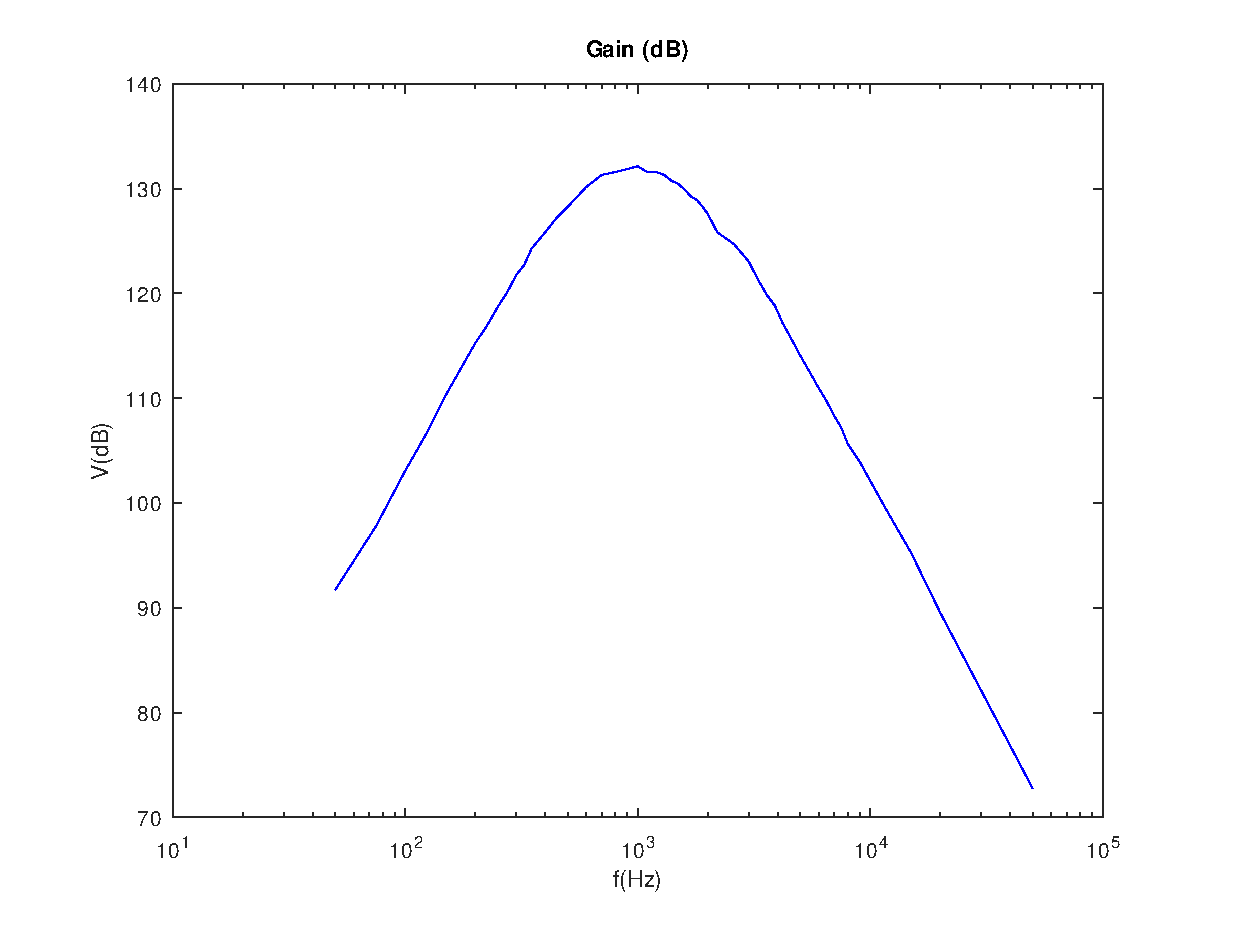
\includegraphics[width=1\linewidth]{lab.eps}